\documentclass[tikz,border=4pt]{standalone}
\usepackage{amsmath,bm}
\usetikzlibrary{arrows.meta,calc,decorations.pathmorphing}
\begin{document}
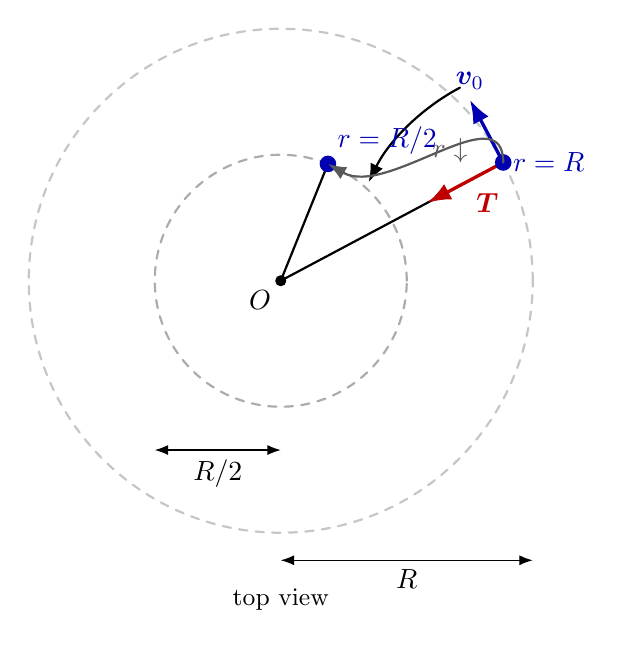
\begin{tikzpicture}[scale=1.0,>=Latex,line cap=round,line join=round]
  \coordinate (O) at (0,0);
  \coordinate (Pi) at (28:3.2);
  \coordinate (Pf) at (68:1.6);

  \draw[gray!45,thick,dashed] (O) circle (3.2);
  \draw[gray!65,thick,dashed] (O) circle (1.6);
  \draw[fill=black] (O) circle (1.8pt) node[below left] {$O$};

  \draw[black,thick] (O) -- (Pi);
  \draw[black,thick] (O) -- (Pf);
  \draw[->,thick] ($(Pi)+(-0.55,0.95)$) arc[start angle=118,end angle=154,radius=2.7];
  \draw[->,very thick,blue!70!black] (Pi) -- ++(118:0.9) node[above] {$\bm v_0$};
  \draw[->,very thick,red!75!black] (Pi) -- ($(Pi)!0.34!(O)$) node[midway,below right] {$\bm T$};

  \fill[blue!70!black] (Pi) circle (3.0pt) node[right] {$r=R$};
  \fill[blue!70!black] (Pf) circle (3.0pt) node[above right] {$r=R/2$};
  \draw[->,thick,gray!70!black] (Pi) to[out=90,in=-30] (Pf);
  \node[gray!70!black] at (2.15,1.65) {$r\downarrow$};

  \draw[<->] (0,-3.55) -- (3.2,-3.55) node[midway,below] {$R$};
  \draw[<->] (-1.6,-2.15) -- (0,-2.15) node[midway,below] {$R/2$};

  \node[align=center] at (0,-4.05) {\small top view};
\end{tikzpicture}
\end{document}
